\section{Optimizador y Algoritmo Genético}
%
% Se seleccionó un algoritmo genético (AG) como método de optimización por ser un
% método sencillo de programar además, este tipo de algorimto es de utilidad
% cuando se tiene una solución con uno o más máximos óptimos locales ó cuando no
% se tiene certeza sobra la suavidad de la función a evaluar.
%

Se seleccionó un algoritmo genético (AG) para realizar la optimización de la
geometría del MRCVC por la simplicidad y facilidad de implementación del mismo.
%
Si bien este tipo de métodos no garantiza que se alcance un resultado óptimo,
en la práctica se ha observado que alcanzan soluciones muy cercanas a las
óptimas tras pocas iteraciones del método~\parencite{goldberg}\parencite{shi}.

Una de las ventajas de este método es que no requiere información del gradiente
de la función que se está evaluando, lo cual es útil cuando no se puede asegurar
la existencia de la derivada de la función en todo el dominio ó cuando se tiene
una función con más de un máximo o mínimo local.
%
Además, el punto de partida de la optimización es una población generada al
azar, se tiene un muestreo aleatorio del dominio que se está evaluando.
%
Esto hace que el método sea poco susceptible a dar como resultado óptimos
locales.

Se puede decir que un algoritmo genético es un método de búsqueda aleatoria
guiada.
%
¿Cómo difieren los AG de los métodos tradicionales de búsqueda?
%
\begin{enumerate}
  \item Los AG pueden operar sobre una representación de las variables estudiadas y
no necesariamente sobre las variables de estudio.
  \item Cada iteración utiliza un conjunto de datos con cierto grado de
aleatoriedad.
  \item Utilizan una función objetivo para evaluar cada punto sin necesidad de
conocer la derivada de la función que se está evaluando.
  \item Los AG usan reglas probabilísticas de decisión.
\end{enumerate}


% \subsection{Componentes básicos de un AG}
%
Los mecanismos básicos que hacen a un algoritmo genético son: 1) SELECCIÓN, 2) CRUZA y 3) MUTACIÓN.
%
El funcionamiento básico se sintetiza en el pseudocódigo~\ref{algo:genetico}.

La SELECCIÓN consiste en crear individuos a partir del puntaje que devuelve
una función objetivo, la cual es la encargada de guiar el proceso de
optimización dando mayor o menor puntaje a un candidato según el resultado que
se quiere obtener.
%
Este paso significa que, aquellos individuos a los cuales se les asignó un
puntaje más elevado tienen más probabilidades de ser copiados o de
``transmitir'' sus parámetros a la iteración siguiente.
%
Este proceso imita en cierta forma la selección natural o evolución Darwiniana y
de aquí viene el nombre de algoritmo genético o evolutivo.

El segundo operador es la CRUZA, consistente en combinar los parámetros de dos
individuos para obtener uno nuevo, esto se asemeja a la reproducción.

Finalmente la MUTACIÓN es la encargada de modificar aleatoriamente uno o más
parámetros de cada nuevo individuo.
%
Este operador juega un rol secundario pero muy importante en la simulación, es
secundario porque se pueden alcanzar soluciones satisfactorias sin que exista la
mutación de la población.
%
Importante porque utilizado con probabilidades pequeñas de ocurrencia, permite
evitar la pérdida temprana de información relevante o convergencia temprana.
%
Por otro lado, en caso de que la probabilidad de mutación sea muy alta, el AG se
convierte en un método de búsqueda aleatoria.

\begin{algorithm} \caption{Algoritmo de optimización}\label{algo:genetico}
  Inicializar población, al azar o a partir de una población ``semilla''.\;
  %
  \While{no se cumpla condición de parada}{
    %
    SELECCIONAR a los individuos más aptos, evaluandolos según la función objetivo.\;
    %
    CRUZAR los candidatos seleccionados para crear la nueva población (la
próxima iteración del método)\;
    %
    MUTAR algunos individuos de la nueva población\;
    %
    \If{se cumple la condición de parada}{
      Parar\;
    }
  }
  {Guardar resultados\;}
\end{algorithm}

%
% \subsection{Implementación}
%
Gran parte de este trabajo consistió en implementar y utilizar a ICESym como LA
función objetivo, aprovechando la cualidad de ``caja negra'' con la que se puede
implementar el simulador.
%
Para lograr esto se modificó parte del código de ICESym con el objetivo de
facilitar la configuración, ejecución y lectura de los resultados que arroja el
simulador y así poder ejecutar de manera automática una simulación con una
configuración particular del motor.
%
Otro aspecto del optimizador que se desarrolló, es el de poder ejecutar
múltiples instancias de ICESym en paralelo con el fin de reducir el tiempo de
ejecución de cada simulación, pudiendo evaluar varios motores (o individuos) al
mismo tiempo.

Para la primera iteración se programaron desde cero los algoritmos y funciones
necesarias para llevar a cabo la optimización con el AG.
%
Posteriormente se tomó la librería DEAP~\parencite{DEAP_JMLR2012} y se
modificaron los operadores a medida, para poder utilizarlos con ICESym.

En los apartados siguientes se describe la implementación de cada uno de los
operadores en el optimizador.

\subsection{Población}
%
Se decidió representar cada motor como un vector con las dimensiones y reglaje
que definen la geometría del sistema de intercambio de gases, los cuales se
listan en la Tabla~\ref{tab:param_motor}.
%
Se limitaron los valores que puede tomar cada parámetro para que la geometría
resultante se asemeje a la geometría del motor utilizado en trabajos anteriores,
aprovechando así los resultados obtenidos en el primer barrido paramétrico.


\begin{table}[ht]
  \centering
  \begin{tabular}{rllll} \toprule
    Nº & Parámetro & Descripción & Sistema & Límites \\ \midrule
    1 & DTA & Diámetro de tubo & Admisión & [60, 100] mm \\
    2 & DTE & Diámetro de tubo & Escape & [60, 100] mm\\
    3 & LIT & Largo de tubo & Admisión & [300, 2000] mm\\
    4 & LET & Largo de tubo & Escape & [300, 2000] mm\\
    5 & IIA & Ángulo geométrico de apertura & Admisión & [0,90]º \\
    6 & IFA & Ángulo geométrico de cierre & Admisión & [IIA, 90]º \\
    7 & IIE & Ángulo geométrico de apertura & Escape & [0, 90]º \\
    8 & IFE & Ángulo geométrico de cierre & Escape & [IIA, 90]º \\ \bottomrule
  \end{tabular}
  \caption{Parámetros que representan al motor}\label{tab:param_motor}
\end{table}


Los vectores que hacen a cada motor se representan como un número binario de 40
dígitos, ocupando 5 dígitos para representar cada uno de los 8 parámetros que
hacen a cada motor.
%
Esto facilita la implementación de los operadores de selección, cruza y
mutación, pudiendo aprovechar implementaciones de operadores existentes en
librerías como DEAP.
%
Estos 8 números binarios luego se convierten en una lista de enteros mediante
una transformación lineal $f(x)=a\cdot x+b$, en la que se ingresa con un entero
entre 0 y $2^{n}-1$ para ir del número binario a un decimal, siendo $n$ la
cantidad de dígitos del número binario (en este caso 5).
%
Los coeficientes $a$ y $b$ son tales que $f(0)=x_{0}$ y $f(2^{n}-1) = x_{1}$,
donde $x_{0}$ y $x_{1}$ son los extremos del rango para el que se quiere aplicar
la transformación.
%
Estos coeficientes ($a$ y $b$) son particulares a cada parámetro, porque se
determinan de acuerdo a los valores que puede tomar cada uno.

De este modo se obtiene el valor de cada uno de los parámetros que hacen a la
configuración particular de cada motor en ICESym.
%
El orden de los mismos se mantiene constante, por lo que cada sección del número
representa una característica en particular del motor.

A modo de ejemplo, en la Figura~\ref{fig:pop_bit} se muestra un número generado
aleatoriamente, la transformada para los primeros 5 dígitos que corresponden al
diámetro del tubo de admisión, 001111.
%
Si se desea que el diámetro del tubo de admisión varíe entre 60 y 100 mm, se
deben obtener los coeficientes $a$ y $b$ para la transformación lineal  a partir
del largo del número binario que se va a utilizar, {\tt{binLen}} y los valores
mínimos y máximos del rango sobre el que se quiere transformar el valor de
entrada: $vMin=60$ y $vMax=100$.

Los coeficientes $a$ y $b$ se obtienen con a partir de:
\begin{align*}
  a &= \frac{vMax-vMin}{2^{binLen} - 1} =\frac{100-60}{2^{5}-1} = 1,2903\\
  b &= vMin=60
\end{align*}

Luego binario transformado a entero vale:
\begin{equation*}
  00111 \longrightarrow 0\cdot 2^{4} + 0\cdot 2^{3} + 1\cdot 2^{2} + 1\cdot 2^{1} + 1\cdot 2^{0} = 7
\end{equation*}

Finalmente, con los coeficientes ($a$, $b$) y el binario transformado en entero,
se tiene que DTA vale

\begin{equation*}
  DTA = a\cdot x + b = (1,2903\cdot 7 + 60) = 69 mm = 0,069 m
\end{equation*}


\begin{figure}[ht]
  \centering
  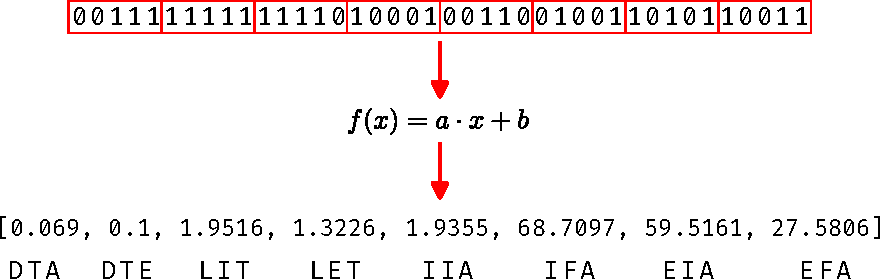
\includegraphics[]{genetico/map_to_engine.pdf}
  \caption{Representación del individuo}\label{fig:pop_bit}
\end{figure}


\subsection{Selección}

Para crear la nueva población se debe elegir a los nuevos candidatos basándose
en los puntajes de la población actual.
%
Hay varios métodos diferentes de selección, como lo son de ruleta, aleatoria,
por puntaje y de tipo torneo.
%
Para este trabajo se seleccionó el método de torneo, es uno de los métodos más
populares para los procesos de selección de AG.

El método consiste en seleccionar $k$ individuos de la población al azar, se
comparan los puntajes de estos individuos y resulta ``ganador'' aquel que tenga
más puntaje.
%
El proceso se repite $N$ veces hasta generar la nueva población.

El parámetro $k$ es el tamaño de torneo y comúnmente se utiliza
2\parencite{oladele}, a mayores valores para $k$ se tiene una mayor pérdida de
diversidad en los resultados\parencite{blickle} porque reduce la posibilidad de
que candidatos con menor puntaje sean seleccionados para la nueva generación
(convergencia temprana).

Para este torneo se utilizó además un \emph{salón de la
fama}~\parencite{wirsansky} de 1 individuo, esto significa que el mejor
individuo de la población actual es automáticamente seleccionado para la
iteración siguiente y la selección por torneo se realiza $N-1$ veces.

\subsection{Cruza}
%
El operador de cruza se encarga de combinar los genes  de dos individuos para
producir uno nuevo.
%
Se encarga de combinar/intercambiar los parámetros de los individuos
``cruzados'' para generar uno nuevo.
%
Para individuos representados por un vector se suelen usar operadores de tipo
cruza de uno o múltiples puntos, también se utilizan mecanismos de cruza
uniforme.
%
El método seleccionado es \emph{cruza de dos puntos}, en este método se corta el
vector que forma al individuo en dos puntos, la posición de estos puntos se
selecciona al azar, manteniendo el largo original de los vectores.
%
Los individuos ``cruzados'' se combinan de forma complementaria como se indica
en la Figura~\ref{fig:cr2puntos}, el algoritmo~\ref{algo:cr2puntos} esquematiza
el proceso.

\begin{figure}[ht!]
  \centering
  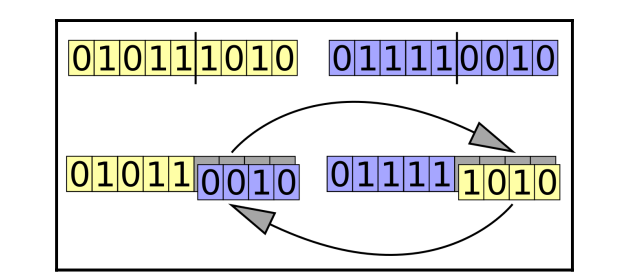
\includegraphics[width=0.5\textwidth]{cruza2puntos.png}
  \caption{Cruza de dos puntos~\parencite{wirsansky}}\label{fig:cr2puntos}
\end{figure}


\begin{algorithm}[h!]
  \KwIn{\\
    $ind_{1}, ind_{2}$: dos individuos de entrada, por ej. [101\ldots011], [110\ldots100].\\
    EA(a, b): devuelve un entero al azar entre los enteros a y b.\\
    L(a): devuelve la cantidad de elementos en a.}
  \KwOut{\\
    $ind_{1}, ind_{2}$: individuos de entrada modificados}
  \SetKwFunction{EA}{EA}
  \SetKwFunction{L}{L}
  % \SetKwFunction{min}{min}
  \BlankLine
  s = min(\L{$ind_{1}$}, \L {$ind_{2}$})\;
  $CX_{1} = \EA{1, s}$\;
  $CX_{2} = \EA{1, s-1}$\;
  \eIf{$CX_{1} \geq CX_{2}$}{
    $CX_{2} = CX_{2}+1$\;
  }{
    $aux=CX_{1}$\;
    $CX_{1}=CX_{2}$\;
    $CX_{2}=aux$\;
  }
  $aux = ind_{1}$\;
  $ind_{1}[CX_{1}:CX_{2}] = ind_{2}[CX_{1}:CX_{2}]$\;
  $ind_{2}[CX_{1}:CX_{2}] = aux[CX_{1}:CX_{2}]$\;
  \Return{$ind_{1}, ind_{2}$}\;
  \caption{Cruza de dos puntos}\label{algo:cr2puntos}
\end{algorithm}

\subsection{Mutación}
%
La mutación juega un rol secundario pero importante en los AG, consiste en
modificar aleatoriamente alguno de los parámetros que definen a un individuo.
%
Este mecanismo contribuye a la diversidad de soluciones y por ende reduce la posibilidad de
convergencia temprana.
%
Se utilizan probabilidades bajas de mutación, en el caso extremo si la
probabilidad de mutación es del $100\%$ el AG se convierte en un método de
búsqueda aleatoria.
%
Algunos de los métodos de mutación utilizados son:

\begin{enumerate}
  \item FLIP BIT
  \item INTERCAMBIO,
  \item INVERSION
  \item REORDENADO ALEATORIO
\end{enumerate}

En este trabajo se utiliza el método de reordenado aleatorio en el cual se
modifica al azar el orden de los números que hacen al individuo, modificando los
índices de la lista que define el arreglo, por ejemplo: $11100 \rightarrow 10011$.
%
El pseudocódigo de este proceso se indica en el algoritmo~\ref{algo:flipbit}.

\begin{algorithm}
  \caption{Flip Bit}\label{algo:flipbit}
  \DontPrintSemicolon
  \KwIn{
    $A = (a_{1}, a_{2}, \ldots, a_{n})$ es un vector compuesto de unos y ceros.\\
    $R$, es una función aleatoria que devuelve un número real entre 0 y 1.\\
    $p$, es un número real entre 0 y 1 que representa la probabilidad de mutación.
  }

  \For{i=1 \KwTo n}{
    \If{$R < p$}{
      \lIf{$A_{i}=1$}{$A_{i}=0$}
      \lElse{$A_{i}=1$}
      }
  }
    \Return A\;
\end{algorithm}

\subsection{Función Objetivo}\label{sec:funcion_objetivo}
%
La función objetivo es la encargada de dar puntaje a los individuos, en la
analogía con la selección natural esta función es el ambiente.
%
Determina la aptitud de un motor con respecto a otro en lo que respecta a
\emph{performance} del sistema de intercambio de gases.
%
Inicialmente se propuso que la función objetivo sea la suma de los rendimientos
volumétricos a todas las velocidades simuladas $s=\sum \eta_{v}$.
%
Este tipo de funciones dió como resultado una curva de $\eta_{v}$ aserrada como
se muestra en la Figura~\ref{fig:curva_aserrada}.

\begin{figure}[ht]
  \centering
  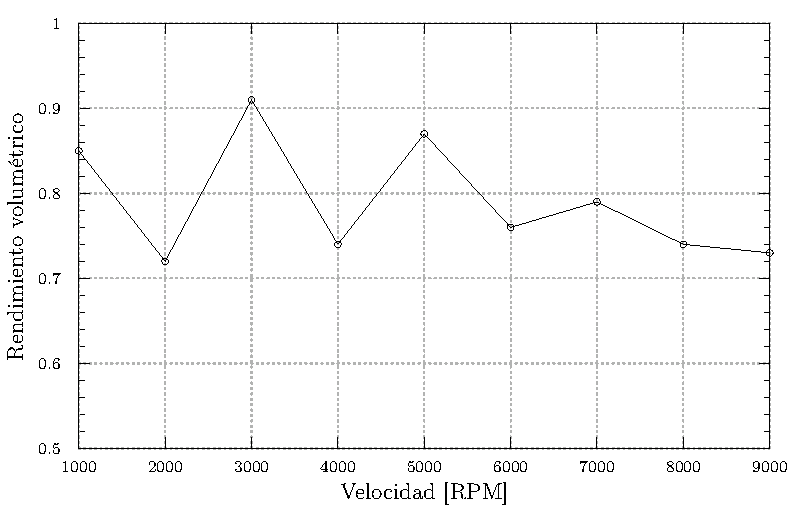
\includegraphics[width=0.7\textwidth]{gnuplot/rendimiento_aserrado.pdf}
  \caption{Curvas de rendimiento volumétrico aserradas}\label{fig:curva_aserrada}
\end{figure}

Esta curva aserrada es poco deseable porque significa una entrega de torque y
potencia dispar, por este motivo se modificó la función objetivo para favorecer
curvas suaves y preferentemente con un solo punto de inflexión.
%
Se implementó una suma ponderada para obtener un rendimiento volumétrico máximo
en un valor cercano a 6000 RPM de modo de aprovechar las características de
balanceo de fuerzas y mayores velocidades de giro de los motores rotativos.
%
La aptitud resulta de la suma del rendimiento volumétrico y el inverso de la
fracción de gases residuales, lo cual probó ser la función objetivo que mejores
resultados dió, la metodología utilizada se resume a continuación.

\begin{enumerate}
        \item Se evalúa cada motor, calculando el rendimiento volumétrico
$\eta_{v}$ y fracción de gases residuales $x_{r}$ para cada velocidad de giro
simulada.
        \item Con $\eta_{v} = (\eta_{v,1}, \ldots ,\eta_{v,n})$ y
$x_{r}=(x_{r,1},\ldots,x_{r,n})$ se hace una suma para cada velocidad
$S_{i}=\eta_{v,i} + x_{r,i}^{-1}$.
        \item Cada motor tiene un vector o lista de valores
$S = (S_{1},\ldots,S_{n})$ para cada velocidad evaluada, con la cual se calcula
el puntaje del motor como:
        \begin{equation}
        f = \sum_{i=1}^{n}{S_{i}} + S_{k}^{2}
      \end{equation}

El valor $S_{k}$ es el puntaje para la $k$-\textit{ésima} velocidad de giro (6000 RPM en
este caso) y se eleva al cuadrado para favorecer altos rendimientos en esta
velocidad.
\end{enumerate}


Durante las primeras iteraciones del método hay una gran cantidad de geometrías
inválidas que devuelven puntaje muy bajo o nulo.
%
En caso de que alguna de las soluciones tenga un puntaje relativamente alto,
existe la posibilidad de una dominancia temprana de la población, provocando
una convergencia temprana de la optimización.
%
Estos candidatos tienen una mayor probabilidad de ``pasar'' sus características
geométricas a las iteraciones siguientes y es algo especialmente problemático en
optimizaciones con poblaciones de alrededor de 100 individuos.

Para reducir la posibilidad de una convergencia temprana se utiliza un método de
escalado de puntajes, que consiste en una transformación lineal en la que se
define el puntaje bruto de un individuo como $f$ y el puntaje escalado como
$f'$, la relación entre ambos es $f' = a\cdot f + b$.
%
Los coeficientes $a$ y $b$ se determinan de modo que $f'_{media}=f_{media}$, de
este modo un motor con puntaje promedio tiene la misma influencia sobre la
población ya sea con la aptitud original o escalada.
%
Para controlar la influencia del mejor individuo de una generación sobre la
próxima, los puntajes se transforman de tal modo que
$f'_{max}=C_{mult}f_{media}$.
%
El valor de $C_{mult}$ es la cantidad de copias que se espera obtener del mejor
de los candidatos en la generación siguiente y se usa en $1,2$ a $2$ para
poblaciones de entre 50 y 100 individuos~\parencite{goldberg}.

Hacia el final donde la diferencia entre puntajes de los individuos de la
población tiende a achicarse, el parámetro $C_{mult}$ cumple la función de
acrecentar las diferencias entre individuos.

En caso de existir individuos con puntaje muy bajo o nulo se hace un
pre-escalado del puntaje que fija el mínimo en $f'_{min}=0$.
%
El procedimiento se lista en los algorimtos \ref{algo:pre-escala} y
\ref{algo:pop_scale}.


\begin{algorithm} \caption{Algoritmo de pre-escalado}\label{algo:pre-escala}
  \KwIn{\\
    $F$, es un vector que contiene los puntajes de todos los individuos\;\\
    $C_{mult}$, es un multiplicador para el escalado, se suele usar
$f\in[1.2, 2]$\;\\ }
  \KwOut{\\
    $a, b$, son los coeficientes para la transformación lineal $f(x)=a\cdot x + b$\;
  }
  \SetKwFunction{max}{max}
  \SetKwFunction{min}{min}
  \SetKwFunction{media}{media}
  \BlankLine

  $u_{max} = \max{F}$\;
  $u_{min} = \min{F}$\;
  $u_{medio} = \media{F}$\;
  \eIf{$u_{min}> aux = (C_{mult}\cdot u_{medio} - u_{max}) \mathbin{/} (C_{mult}-1)$
    }{
    $\Delta_{u} = u_{max}-u_{avg}$\;
    $a = (C_{mult} - 1) \cdot u_{avg} / \Delta u$\;
    $b = u_{avg} \cdot (u_{max} - C_{mult} \cdot u_{avg}) \Delta_{u} $\;
  }{
    \eIf{$\Delta \neq 0$}{
      $a = u_{avg} \mathbin{/} \Delta_{u}$\;
      $b = -u_{min} \cdot u_{avg} \mathbin{/} \Delta_{u}$ \;
    }{
      $a=1$\;
      $b=0$\;
    }
  }
  \Return{$a, b$}
\end{algorithm}


\begin{algorithm}\caption{Escalado de población}\label{algo:pop_scale}
  \KwIn{\\
    $f$, es la aptitud.\\
    $a, b$, son los parámetros de la función de pre-escalado. \\
  }
  \KwOut{\\
  $f^{*}$, los puntajes escalados.}
  \SetKwFunction{ps}{PreEscalado}
  \SetKwFunction{ll}{Largo}
  \SetKwFunction{esc}{Escala}
  \BlankLine

  $a, b = \ps{f, 2}$\;
  $f^{*} = ()$ \;
  $n = \ll{f}$\;
  \For{$i=1$ \KwTo $n$}{
    $f^{*}_{i} = a\cdot f_{i} + b$\;
  }
  \Return{$f^{*}$}\;
\end{algorithm}

% Con la población definida se procede a los evaluar cada motor con la función
% objetivo, la cual se definió de manera tal de favorecer curvas de rendimiento
% volumétrico suaves y valores altos a mayores RPM.\@

% La suavidad de la curva de rendimiento volumétrico se calcula midiendo los
% cambios de pendiente de la derivada la cual se aproxima con la fórmula de
% diferencia progresiva~\ref{eq:derivada}.
% %
% Solamente interesa el signo, por lo que el valor de $h$ en el denominador no
% interesa y se hace 1, con esto la función objetivo queda como el
% algoritmo~\ref{alg:funcObj}.

% \begin{equation}\label{eq:derivada}
%   f' = \frac{f(i+1) - u(i)}{h}
% \end{equation}

% Una vez evaluados todos los motores de la población, se debe seleccionar los
% individuos que formarán la siguiente iteración del algoritmo.
% %
% El método de selección es de tipo TORNEO, en el cual se seleccionan los mejores
% $k$ individuos de un grupo al azar de $N$ candidatos.
% %

% Con los nuevos candidatos seleccionados, se procede a variar la población,
% realizando la cruza y mutación.

% Luego se toman pares de individuos y de acuerdo a la probabilidad de cruza, se
% combinan con el método seleccionado.

% Finalmente se realiza una segunda iteración sobre la nueva población, aplicando
% el método de mutación a cada individuo, de acuerdo a la probabilidad de
% mutación indicada.
%
